\documentclass{standalone}

\usepackage[euler-digits]{eulervm}

\usepackage{tikz}
\tikzset{every node/.style={circle,draw,minimum size=6mm,inner sep=0pt}}

\begin{document}
    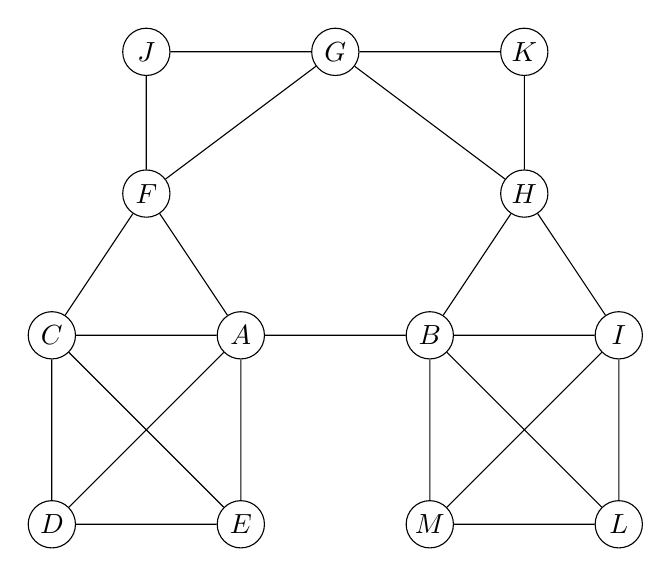
\begin{tikzpicture}[scale=1.2]
      \node (A) at (-1,2) {$A$}; 
      \node (B) at (1,2) {$B$}; 
      \node (C) at (-3,2) {$C$}; 
      \node (D) at (-3,0) {$D$}; 
      \node (E) at (-1,0) {$E$}; 
      \node (F) at (-2,3.5) {$F$};
      \node (G) at (0,5) {$G$};
      \node (H) at (2,3.5) {$H$};
      \node (I) at (3,2) {$I$};
      \node (J) at (-2,5) {$J$};
      \node (K) at (2,5) {$K$};
      \node (L) at (3,0) {$L$};
      \node (M) at (1,0) {$M$};

      \draw (A) -- (B);
      \draw (D) -- (C) -- (F) -- (A) -- (E) -- (D) -- (A) -- (C) -- (E);
      \draw (L) -- (I) -- (H) -- (B) -- (M) -- (L) -- (B) -- (I) -- (M);
      \draw (F) -- (G) -- (H) -- (K) -- (G) -- (J) -- (F);
    \end{tikzpicture}
\end{document}
